%FROM SANGBAEK
During RG-A data taking, the event was triggered in parallel by three physics trigger systems: (1) the electron trigger, (2) photoproduction trigger and (3) opposite sector trigger. This analysis focuses on the (inclusive) electron trigger that is designed to record events with FD electron candidates with minimum $n_{phe}$, $E_{dep.}$, $E_{dep.} PCAL$ conditions and the geometrical matching between detector subsystems. The electron trigger search was adjusted and performed in parallel for each sector. The electron trigger system is highly efficient with 99.5\% trigger efficiency and 95\% DAQ livetime for trigger electrons of momentum above 2 GeV/c. The desired event rate for the RG-A experiment is about 20 kHz, which was estimated using the simulation. This can be easily achieved by the CLAS12 trigger logic with the effective performance level up to 200 kHz \parencite{Raydo2020TheSystem}. The events triggered by the electron trigger has trigger bits ``1'' (True) in any of bits 0 to 6, where the bits 1–6 stan for each sector and 0 is their OR. The trigger bits can be accessed offline. Processing all saved inclusive events is not efficient in many aspects. There are a lot more inclusive events than the exclusive channels of interest, namely DVCS and DV$\pi^0$P. The RG-A has a few skimming modes, trains and wagons, to be commonly used for some specific channels. A train is a coarse skimming, such as the inclusive skim, which requires an electron-proton pair in one event. A wagon is a relatively finer skimming, such as the DVCS wagon, which requires one electron-proton-photon set with some level of DVCS exclusivity. The series of skimming processes is called data cooking. In this analysis, for the base data set we take the DVCS wagon that selects the DVCS candidates with loose exclusivity cuts, and require at least one $e'p'\gamma$ set in the event \sangsite{158} (see Section 3.3 for the cut conditions). The raw data is stored in the HIPO format \sangsite{151} for the entire CLAS collaboration. The HIPO format has the advantages of fast Input/Output (I/O) speed, and compatibility with the Event I/O (EVIO) format that is commonly used for the Jefferson Lab event storage  \parencite{Wolin2007EVIOPackage}. For this analysis, the python program with pandas library was taken as the main analysis tool in that python is supported by modern statistical packages \sangsite{160,161} that are well maintained. This motivates operation of a custom pipeline to convert the data format to pickle, which is the python standard data format \sangsite{162}. We use the CLAS12ROOT \sangsite{163}, a software package to read the HIPO format in C++ and store the related information in ROOT format \sangsite{164}. The ROOT formatted data is once again converted to pickle format, using the uproot library \sangsite{165}. By doing so, the data are reduced into $M \times N$ dimensionality, where $M$ is the number of events, and $N$ is the number of physical quantities and other information that are related (Fig. 2-16). Different data formats have advantages in different stages of data processing. We filter the base data with the PID cuts introduced at Section 2.4 and save in another HIPO format, because the base data contains all detector responses. The filtered HIPO files are converted into ROOT format. Finally, we execute the python script to select DVCS and DV$\pi^0$P events with tighter Event Selection criteria that will be described at 3.3 and save them in the pickle format.



Cooked hipo - PID cuts - filtered hipo - converting - converted root - dvep cuts - exclusive pickle

An electron candidate e'is defined as an associated signal of these FD signals: (1) a track in DC, (2) photoelectrons in HTCC, (3) hits in FTOF, (4) energy deposited over 60 MeV, and (5) the Sampling Fraction (SF) of Minimum Ionizing Particle’s (MIPs). Here, the event start time is determined from the track information, and corrected by the RF signal and the vertex location. The momentum of a charged particle such as e' and the proton p' is reconstructed using the equation of motion in a magnetic field. The polar angle difference during the trajectory $\Delta \theta$ is related to the momentum p and the charge q of the particle, and the line-integrated magnetic field along the trajectory curve, (int B dl) as

\begin{equation}
    \frac{q}{p} = \frac{\Delta \theta}{c \int B dl}
\end{equation}

During one event, p' is identified when there is a positively charged track in the DC
or the CVT, associated with FTOF or CTOF hits for the timing. The flight time $\Delta t_{p'}$ of p' is determined as the difference of TOF hits and event start time. Along
with the path length $l_{p'}$ and the momentum $p_{p'}$ determined from the trajectory, the following relationship holds [151];

\begin{align*}
    \beta p' &\equiv \frac{v p'}{c} = \frac{l p'}{c t p'} = \frac{p'}{\sqrt{p'^2 + M^2 p}}
\end{align*}

We take the common relativity notation for $\beta = \frac{v}{c}$ where $v$ is the velocity of the particle and $c$ is the speed of light. Here, $\chi \equiv \frac{\Delta t}{\sigma TOF}$ with $\Delta t \equiv \Delta t_{p', \text{expected}}(p') - \Delta t_{p', \text{measured}}$ is assigned to the particle as the signed distance function from the theoretical value. The photon $\gamma$ can be reconstructed in the ECAL in FD, and the FT-Calorimeter in the FT. A photon will not produce charged tracks in the DC and the FT-Hodo associated with the existing calorimeter hits. More efficiently, the neutral hits are defined as the remaining calorimeter hits after all charged particles are assigned. The energy deposition in ECAL is converted to the actual photon energy using the SF. The homogeneous calorimeter FT-Cal takes the energy deposition as the photon energy.


    \begin{figure}[H]
        \centering
        \subfloat[]{
            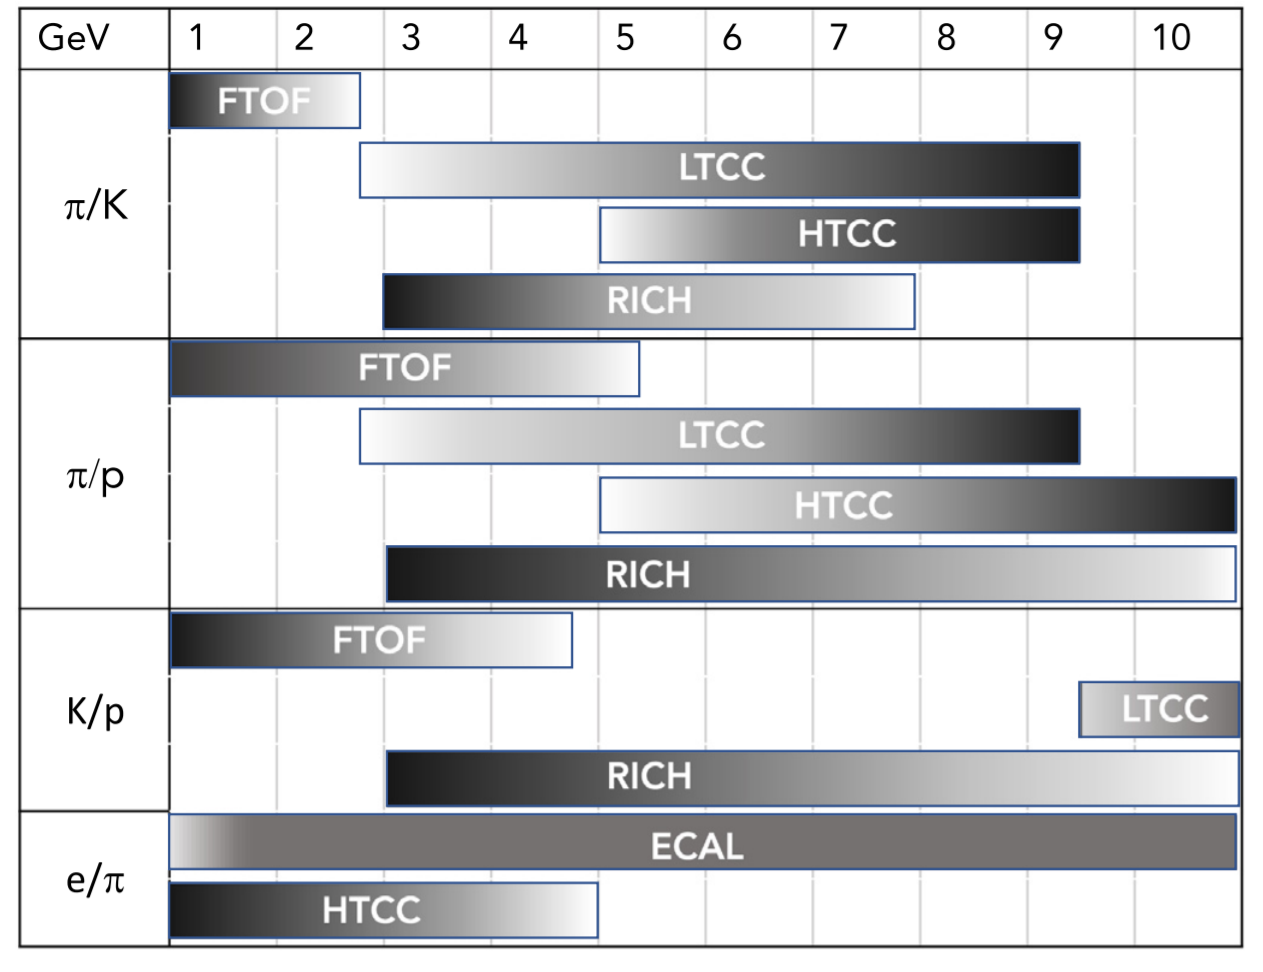
\includegraphics[width=0.3\textwidth]{Chapters/Ch2-Experiment/clas-12-exp/clas-detectors/other/pics/pid-clas12.png}
        }
        \caption{Your caption goes here}
        \label{fig:clas12-pid-overview}
    \end{figure}

    
The Data Acquisition (DAQ) \parencite{Boyarinov2020TheSystem} 


\iffalse

Sangbaek refs:
133 - pac approval rga 
134 - jlab schematic 
143 - FMT 
147 - FT 
149 - Faraday cup 
150 - DAQ 
151 - magnet relationships
152 - forward calorimeter 
153 variou channel analysis
154 variou channel analysis
155 variou channel analysis
156 - PCal boundary estimation - FX private comm
158 - DVCS conditions - F.-X. Girod et al., DVCS Wagon, 2020
160 - stat packages
161 - stat packages
162 - pickle format The Python Library Reference, Release 3.8.2.
163 - clas12rot D. Glazier et al., CLAS12ROOT
164 - root Root-project/root: V6.18/02,
165 - uproot Scikit-hep/uproot:

\fi


\begin{figure}
    \centering
    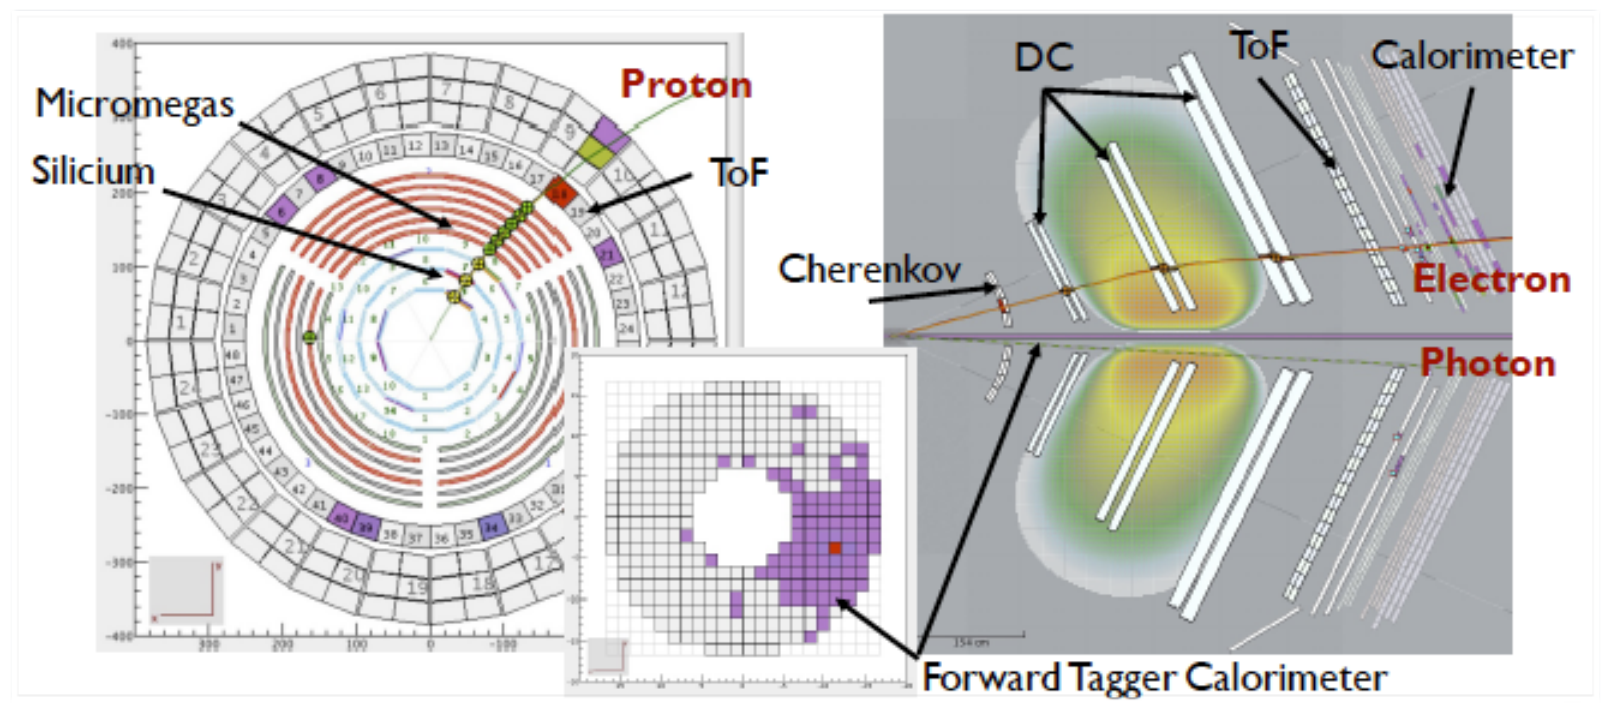
\includegraphics[width=0.9\textwidth]{Chapters/Ch2-Experiment/recon_pid/pid_figs/example_track.png}
    \caption{Caption from \parencite{Battaglieri2021PresentProgram}}
    \label{fig:example-track}
\end{figure}


here we talk about CLAS PID




cross section that requires the coincidence detection of electron, proton,
and photon.

\subsection{Decoding and Track Reconstruction}\label{sec:decrec}

\subsection{Particle Identification}
**photon cuts:
pid 22, status > 2000 (in FD or CD, not ftagger)
momentum greater than 400 MeV each

**proton cuts: pid 2212

**electron cuts: pid==1 and status < 0(negative particle

sangbaek lee thesis \parencite{Lee2022MeasurementDetector}

For this analysis all final state particles should be detected.
After $\pi^0$ decay we are going to have 4 particles: electron, proton and two photons.
The particle identification methods are applied to select the exclusive event with at least one electron, proton and two photons. 


    \subsubsection{Electron}
    \subsubsection{Proton}
    \subsubsection{Photon}
    \subsubsection{Pion}
    
    Basic event builder cuts are utilized, then additional cuts are made that are common with the RGA Analysis note (\href{https://www.overleaf.com/project/5ea737720942930001ff5e9c}{overleaf link} and developed by Sangbaek Lee (sangbaek@mit.edu - \href{https://github.com/Sangbaek/analysis_code/tree/analysis/pid}{github code here}. For this analysis, both the central detector and forward detector are utilized for proton tracking. The forward tagger is also utilized for photon identification. 
    


    In addition to individual particle PID procedures the cut on the mass of two photons is applied:
    \begin{itemize}
    	\item $0.07<M_{\gamma\gamma}<0.2$ GeV
    \end{itemize}
    The pion is more thoroughly constrained by the exclusivity cuts, described in the next section.
    

\begin{figure}[hbt]
	\centering
	\includegraphics[page=6,width=0.6\textwidth]{Chapters/Ch2-Experiment/recon_pid/pid_figs/eppi0.exclusive.pdf}
	
	\caption{The distribution for mass of two photons $M_{\gamma\gamma}$}.
	\label{fig:ggmass}
	
	\centering
	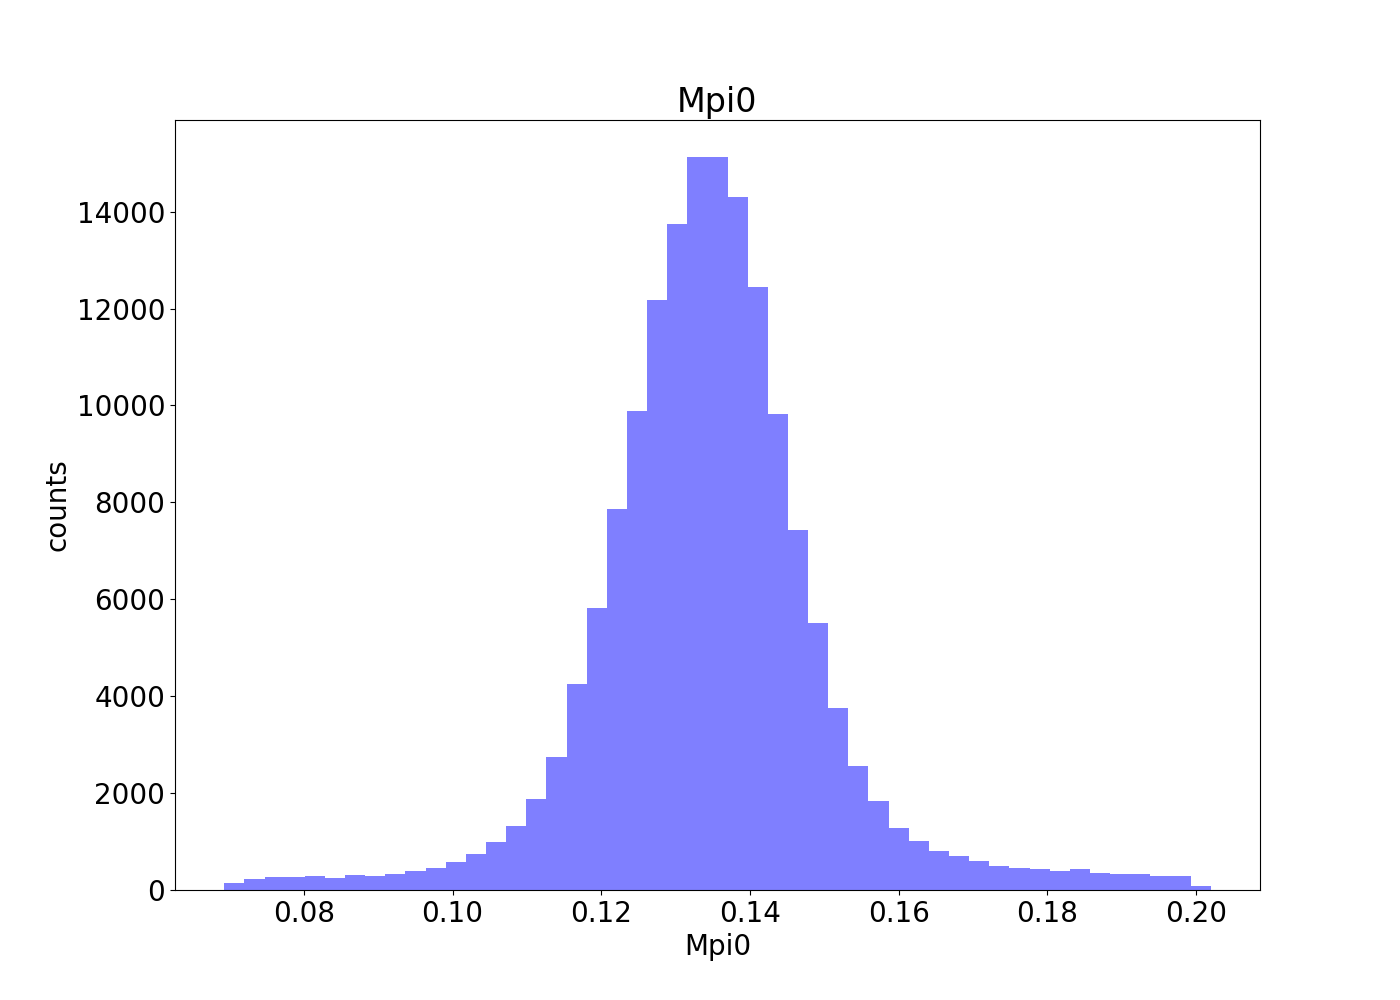
\includegraphics[width=0.6\textwidth]{Chapters/Ch2-Experiment/recon_pid/pid_figs/Mpi0.png}
	
	\caption{The distribution for mass of two photons after exclusivity cuts}.
	\label{fig:ggmass_after}
	
\end{figure}




\subsection{Data Storage and Formatting}
    \subsubsection{Data Location and Availability}
    \subsubsection{File Formatting and Conversion}\label{sec:filtering}
        Mention that same transformations are used for rec events and filtering
    
